\section{Zusammenfassung}
\label{sec:Zusammenfassung}
Die Simulation zeigt auf, wie viele Faktoren Einfluss auf die Wassertemperatur haben. Der Wärmeverlust erfolgt unter anderem über die Wände des Pools (Wärmeleitung), über den Wärmeaustausch zwischen Luft und Wasser (Konvektion) und über Verdampfung (Evaporation). Dies sind die Faktoren, gegen welche sich die Heizung und die Sonneneinstrahlung behaupten müssen, um den Pool auf eine Badetemperatur von 30\,°C zu erwärmen. Die Simulation veranschaulicht den Einfluss der verschiedenen Faktoren auf die Pooltemperatur.

Überraschend war die Erkenntnis, dass der Wärmeverlust durch Konvektion einen derart grossen Einfluss (bei 30\,°C etwa 60.8\,\%) hat. Der Verlust über die Wände und den Boden haben wir in der gefundenen Grössenordnung erwartet. Die Temperatur der Erde unterliegt nur geringen Schwankungen und die Wärmeleitung über die isolierten Wände erfolgt sehr träge.

Die Herausforderung der Simulation lag vorwiegend im theoretischen Bereich. Um die Teilsysteme zu verstehen, mussten wir uns mit physikalischen Berechnungen aus dem Bereich Wärme und Strahlung auseinandersetzen.


\begin{figure}[H]
	\centering
	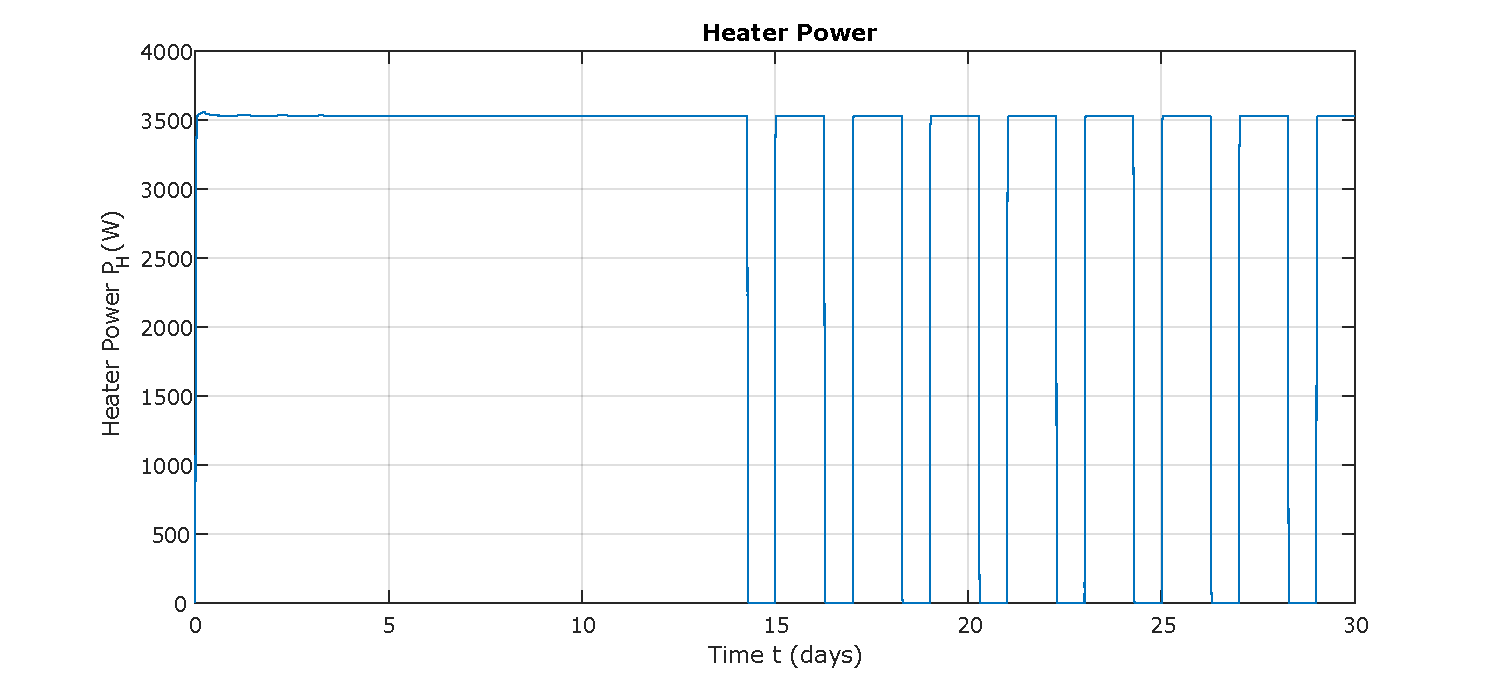
\includegraphics[width=\linewidth]{heizung}
	\caption{}
	\label{fig:heizung}
\end{figure}

\begin{figure}[H]
	\centering
	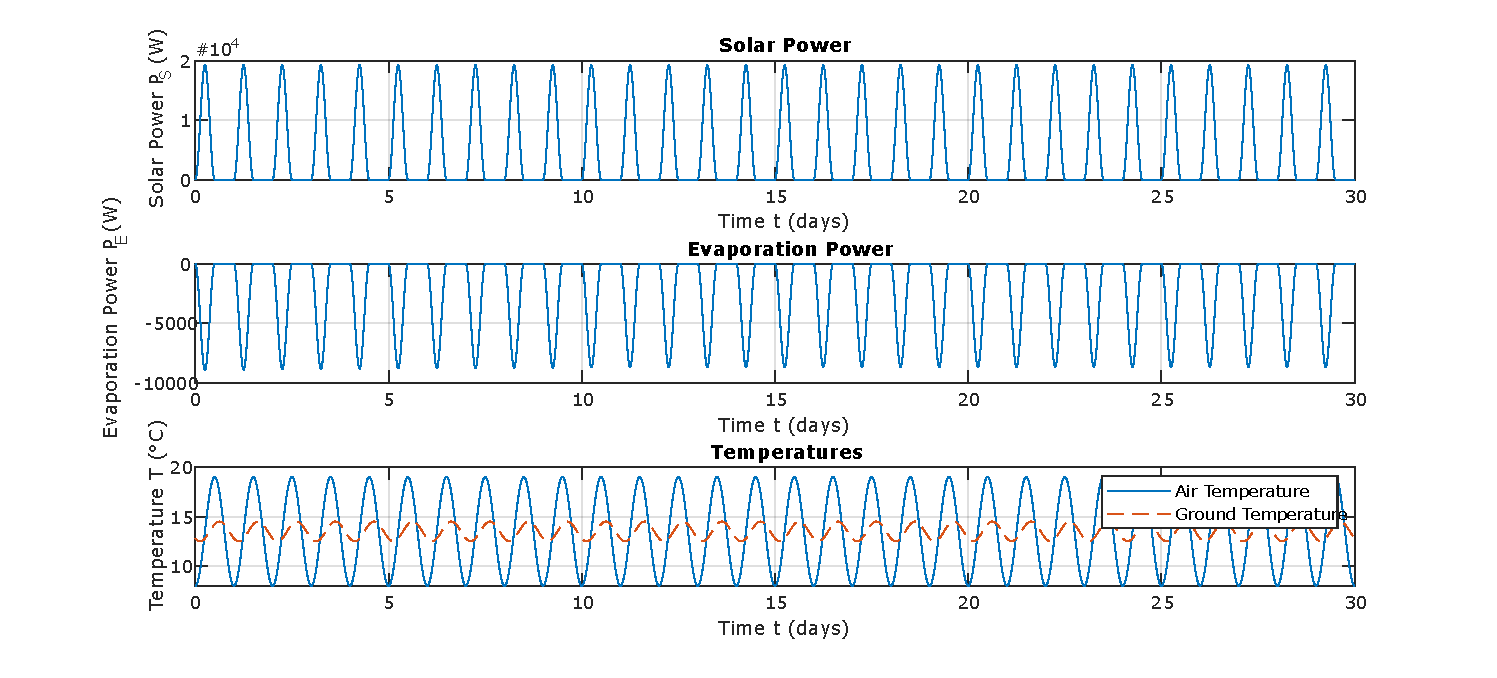
\includegraphics[width=\linewidth]{umgebung}
	\caption{}
	\label{fig:umgebung}
\end{figure}

\begin{figure}[H]
	\centering
	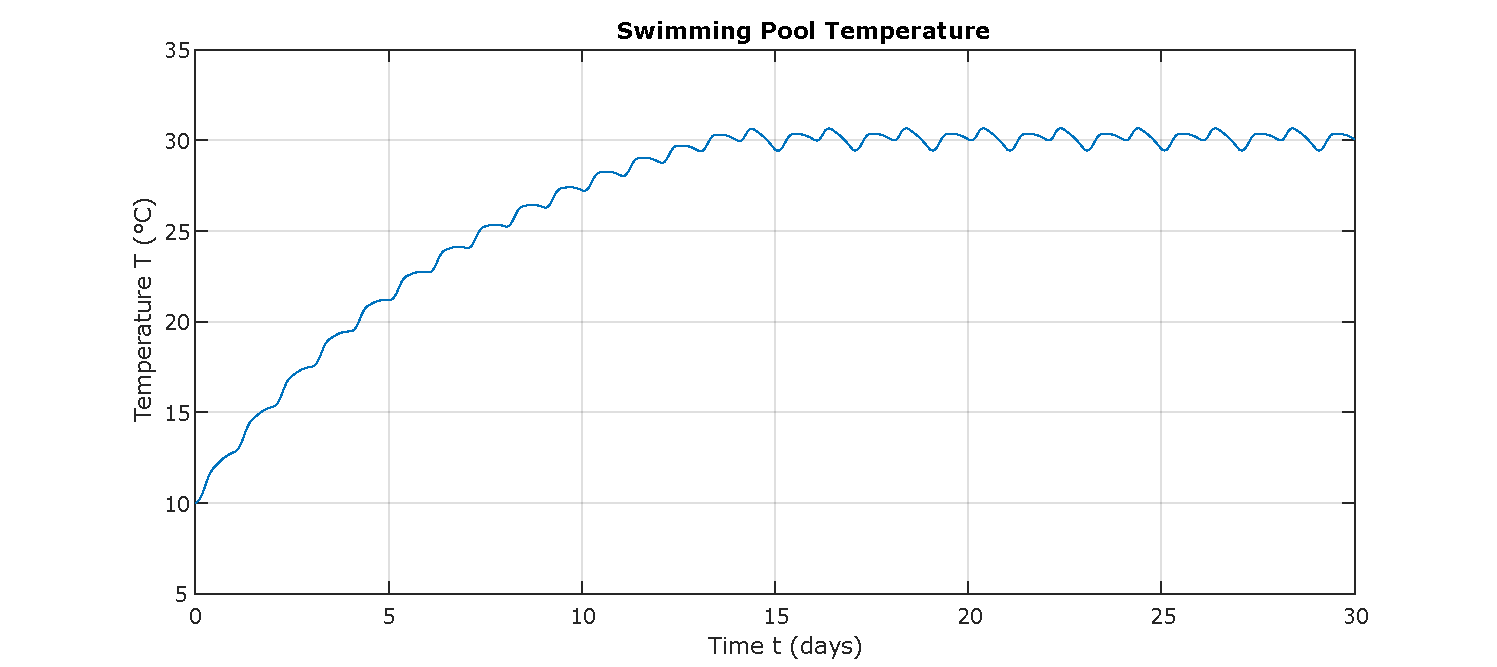
\includegraphics[width=\linewidth]{pool-temp}
	\caption{}
	\label{fig:pool-temp}
\end{figure}

\begin{figure}[H]
	\centering
	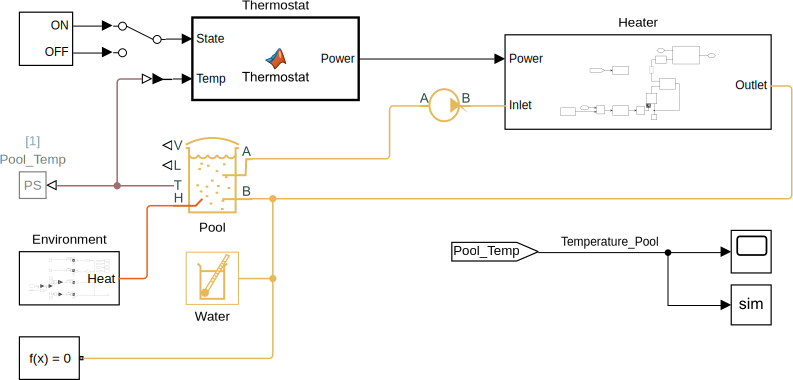
\includegraphics[width=\linewidth]{SwimmingPoolSimulationModel}
	\caption{}
	\label{fig:SwimmingPoolSimulationModel}
\end{figure}
\begin{figure}[H]
	\centering
	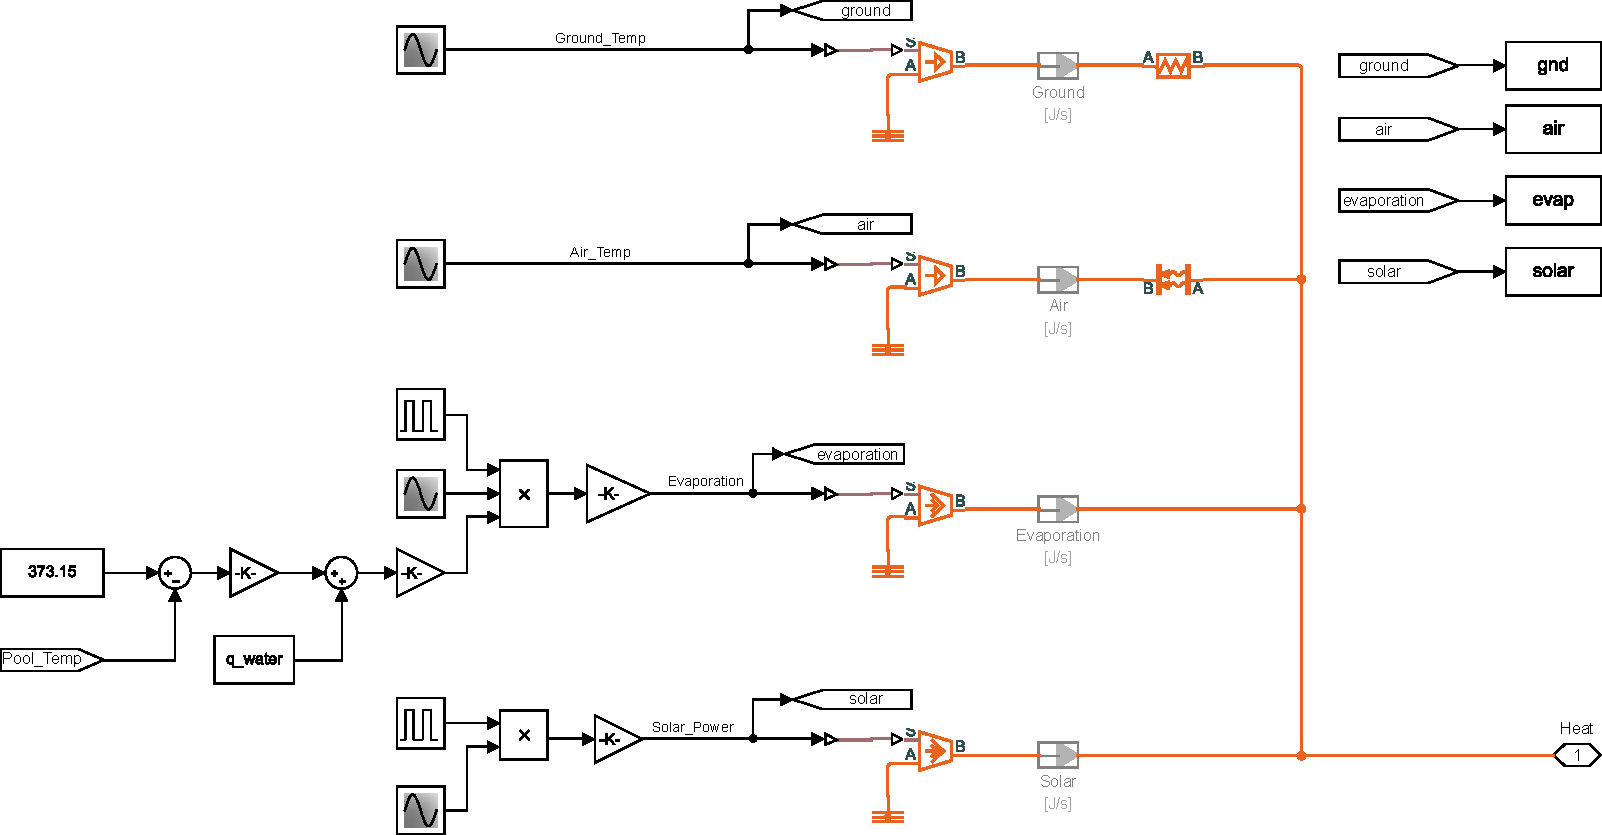
\includegraphics[width=\linewidth]{EnvironmentModel}
	\caption{}
	\label{fig:EnvironmentModel}
\end{figure}

\begin{figure}[H]
	\centering
	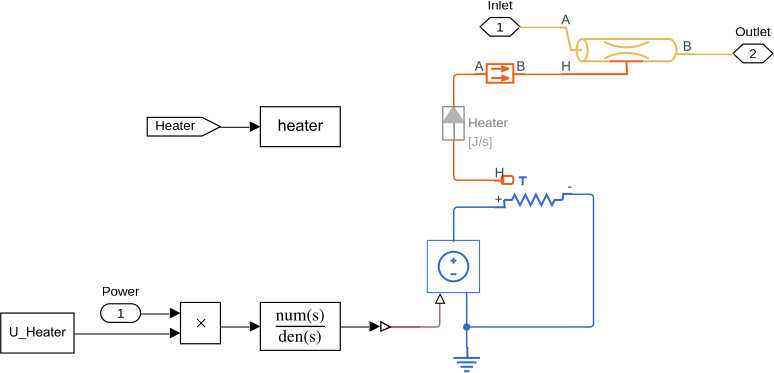
\includegraphics[width=\linewidth]{HeaterModel}
	\caption{}
	\label{fig:HeaterModel}
\end{figure}


